\documentclass{article}
\usepackage[utf8]{inputenc}
\usepackage{graphicx}
\usepackage{amsmath}


%%%%%%%%%%Positioning of graphics figures
\usepackage{float}
\usepackage{subcaption}
\usepackage{amssymb,amsthm,amsmath}   
\graphicspath{{0_images/}}
\usepackage{geometry}
\usepackage[breaklinks]{hyperref}
\usepackage[table,xcdraw]{xcolor}


%Adding bibliography to table of contents
\usepackage[nottoc]{tocbibind}
%Adding bibtex reference file
\usepackage[backend=biber,sorting=ynt]{biblatex}
\addbibresource{references.bib}


%Custom file where we put terms and definitions
\usepackage{terms}
\setlength\parindent{0pt}

%Custom command for commenting out multiple lines
\newcommand{\comment}[1]{}

%Abbreviations package
%\usepackage[acronym]{glossaries}

%Center figure and table captions
\usepackage{caption}

%Formatting code
\usepackage{listings}
\lstset{
    inputencoding=utf8,
    extendedchars=true,
    literate=   {"}{{\\o}}1
                {ä}{{\"a}}1
                {ü}{{\"u}}1
}





\begin{document}

\begin{titlepage}
\center % Center everything 
\textsc{\LARGE Danmarks Tekniske Universitet}
\\[1cm]
\textsc{\huge{Bachelor Project}}
\\[1cm]
\begin{figure}[H]
    \centering
    
\includegraphics[width=10em]{dtu_logo.png}
\end{figure}
\\[2cm]
\textsc{\huge{Scalable Machine Learning}}
\\[0.5cm] 
\textsc{\huge{for}}
\\[0.5cm] 
\textsc{\huge{Temporal Dynamic Graph Networks}}
\\[1.0cm]
\textsc{August Semrau Andersen - s183918
\\ William Diedrichsen Marstrand - s183921} 
\\[10pt]
%\textsc{\LARGE } \\ \textsc{\LARGE} \\[0.5cm]
%\includegraphics[width=9.5cm]{images/}

\medskip
%Number of characters: 12600, Standard Pages: 5.25
\null
\vfill
\vspace{0.5cm}
\begin{center}
\today,
 Danmarks Tekniske Universitet\\
\end{center}
\end{titlepage}


\newpage
\pagenumbering{gobble}


\subsection*{Abstract}

This project proposes the Stepwise Constant Velocity Model (SCVM) which models dynamic networks in two-dimensional latent space using Newtonian dynamics with stepwise computation.
The SCVM was implemented with a vectorized training setup in order to utilize the power of CUDA that stems from parallelization.

The proposed model was evaluated in terms of modelling capabilities, and was found to model dynamic networks well, using Newtonian dynamics in a stepwise fashion as to accommodate for the 

Running times were evaluated for the SCVM running on CPU and CUDA, the results concluding that vectorized training setup greatly improves running times when utilizing CUDA.
This scalable implementation enabled for the modelling of larger dynamic networks than would have been feasible with a non-parallelized training setup.

The learned Newtonian dynamics of a given dynamic network were visualized via the creation of animation which depicted the stepwise constant velocity movements of nodes in latent space.
These animations were improved through the implementation of non-disruptive corrections to the learned dynamics, elevating the interpretability and explainability of the modelled dynamic network.


The paper discusses these results and argues for the investigation of number of aspects of the proposed SCVM which could improve its modelling capabilities, scalability and the explainability of resulting visualizations.

Lastly, possible use cases for the proposed model are discussed, amongst which 



\newpage
\pagenumbering{arabic}

\tableofcontents
\clearpage

\comment{
\makeglossaries
\newacronym{vc}{VC}{Voice Conversion}
\newacronym{stt}{STT}{Speech-To-Text}
\newglossaryentry{vcmodel}
{
        name=VC model,
        description={Is a model that converts one speakers voice to another speakers voice.}
}

\newglossaryentry{sttmodel}
{
        name=STT model,
        description={Is a model that transcribes spoken words into written words.}
}

\printglossary[type=\acronymtype]
\printglossary
}




%%%%%%%%%%%%%%%%%%%%%%%%%%%%%%%%%%%%%%%%%%%%%%%%%%%%%%%%%%%%%%%%%%%%%%%%%%%%
%%%%%%%%%%%%%%%%%%%
\section*{Acronyms}

\textbf{CVM} - Constant Velocity Model
\\\\
\textbf{SCVM} - Stepwise Constant Velocity Model
\\\\
\textbf{TDGN} - Temporally Dynamic Graph Network
\\\\
\textbf{PP} - Possion Process






%%%%%%%%%%%%%%%%%%%
%\section*{Glossary}

%\textbf{VC model} - Is a model that converts one speakers voice to another speakers voice.
%\\\\
%\textbf{STT model} - Is a model that transcribes spoken words into written words.

%\printglossary[type=\acronymtype]
%\printglossaries
%\section*{Glossary}
\clearpage

\section{Introduction}
\label{sec:Intro}

This section introduces the project, it's motivations and scope.
It will lightly shed light on the technical background of the project, introducing machine learning on graph networks.
The main research questions will be outlined, and a review of related work will follow.
Lastly, an overview of the contents of the project will be given.
\\\\
All code for the project is publicly available at \href{https://github.com/TGML-Bachelor-Project/TGML}{\textcolor{blue}{https://github.com/TGML-Bachelor-Project/TGML}}


%%%%%%%%%%%%%%%%%%%%%%%%%%%%%%%%%%%%%%%%%%%%%%%%%%%%%%%%%%%%%%%%%%%%%%%%%%%%%%%%%%%%%%%%%%
\subsection{Motivation and Purpose}
\label{sec:Intro:Motivation}

%%%%%%%%%%%%%%%%%%%%%%%%%%%%%%%%%%%%%%%%%%%%%%%%%%%%%%%%%%%%%%%%%%%%%%%%%%%%%%%%%%%%%%%%%%
\subsection{Problem Statement}
\label{sec:Intro:ProblemStatement}


%%%%%%%%%%%%%%%%%%%%%%%%%%%%%%%%%%%%%%%%%%%%%%%%%%%%%%%%%%%%%%%%%%%%%%%%%%%%%%%%%%%%%%%%%%
\subsubsection{Research Questions} 
\label{sec:Intro:ResearchQs}
To guide the investigation a set of research questions have been formulated.
\\\\
\textbf{Main Research Question}
\\
How can a scalable and explainable model be implemented for visualizing interactions in a temporal dynamic graph network?
\\\\
\textbf{Sub-Questions}
\begin{itemize}
    \item How well can TDGNs be modelled using a velocity-dependant representation in latent Euclidean space, with stepwise event computation, and how well can it model the evolution of the TDGNs?
    
   \item To what extend can the model be implemented in a scalable manner?
   
   \item How can the model be visualized to enforce explainability?
   
\end{itemize}


%%%%%%%%%%%%%%%%%%%%%%%%%%%%%%%%%%%%%%%%%%%%%%%%%%%%%%%%%%%%%%%%%%%%%%%%%%%%%%%%%%%%%%%%%%
\subsection{Related Work}
\label{sec:Intro:RelatedWork}




%%%%%%%%%%%%%%%%%%%%%%%%%%%%%%%%%%%%%%%%%%%%%%%%%%%%%%%%%%%%%%%%%%%%%%%%%%%%%%%%%%%%%%%%%%
\subsection{Bachelor Project Outline}
\label{sec:Intro:ThesisOutline}









\clearpage



\section{Method}
\label{sec:Method}
This section will delve with the technical methodology used in this project.
\\
First, it will give an explanation of the graph networks in the context that this project utilizes. 
\\
It will then explain the central idea behind the velocity dependant model about which the project revolves. 
\\
From there, this section will dive deep into the different aspects that this model relies upon.
This both includes mathematical and statistical theory, as well as the methodology related to implementing the model in code.

\subsection{Graphs and Networks}
\label{sec:Method:Graphs}
The most common way of describing a network of anything, that could be of accounts on Facebook, the electrical grid, distribution of goods from warehouses to stores etc. is to use a graph.
A graph is a representation that consists of a set of $N$ nodes, the entities whose interactions we are trying to depict, and edges $E$ which represent said interactions.


\subsubsection{Static Graphs}
\label{sec:Method:Graphs:StaticGraphs}
The most common type of graph is the static graph with a representation of nodes and edges that never changes. 
In this way, the static graph can be seen as a snapshot of a given network at a single point in time.

A static graph representation of the relationships between characters in the book series 'Harry Potter', can be seen in figure \ref{fig:StaticGraph}.

\begin{figure}[H]
    \centering
    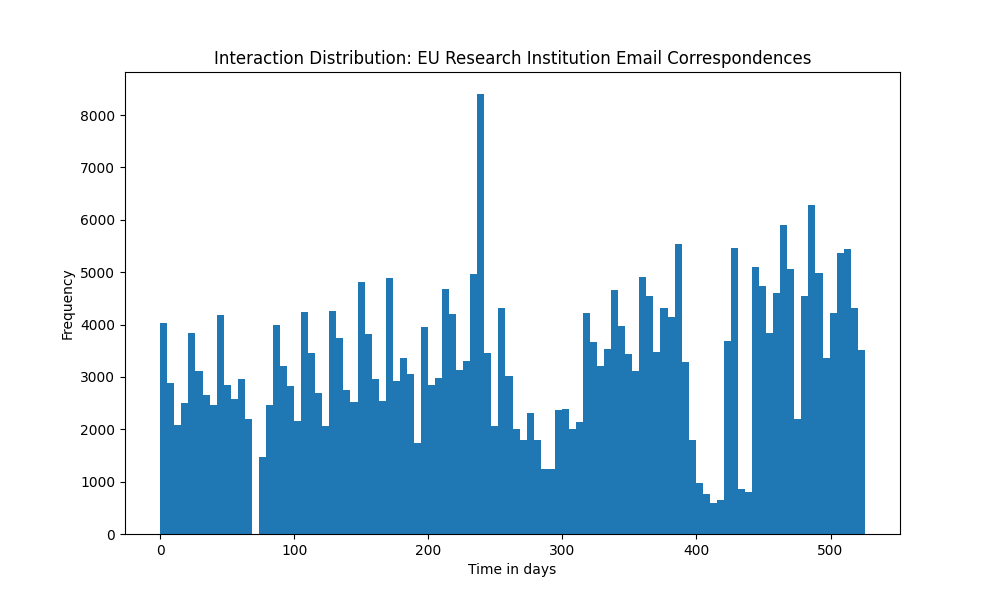
\includegraphics[width=\textwidth]{0_images/reallife_dataset_2_dist.png}
    \caption{A static graph representation of the relationships between characters in the book series 'Harry Potter'. Each node represents a specific character, that can be Hermione Granger, Ron Weasly or Harry Potter himself, and the edges that connect them represent the fact that a given pair of characters have interacted directly during the book series}
    \label{fig:StaticGraph}
\end{figure}


\subsubsection{Temporally Dynamic Graphs}
\label{sec:Method:Graphs:DynamicGraphs}
Not all networks can be represented by static graphs though, and sometimes having graphs be non-static means that they make for a better representation of the network they are modelling. 
When talking about temporally dynamic graphs, this project refers to graphs that are subject to a sequence of \textit{updates} over time. 
An update is an action that \textit{inserts} or \textit{deletes} edges or nodes in the graph or actions that \textit{alter attributes} of nodes or edges.


The dynamic aspect differ between graphs, as they can be changing in different dimensions. 
This project focuses entirely on the very commonly used graphs that are dynamic in the temporal dimension, \textit{temporal dynamics graphs}, i.e. they change over time, this is not always the case. 
Another example could be if we had a network representing the airports which a plane could directly fly to. 
Now the graph would be dynamic in the geographical position of the plane as the graph could change to show which airport the plane is connected to based on its current position. 
Say the graph for the plane being at the Reykjavik Airport on Iceland will then change when the plane gets to Los Angles.












\subsection{Constant Velocity Model}
\label{sec:Method:VModel}

This subsection will describe the idea of the Constant Velocity Model, on which the Piecewise Constant Velocity Model is based, and lightly explain the theoretical aspects enabling its workings.
The section will not dive into the technical aspects of how it works, as these will be delved with in the following sections.
Instead, it serves as the foundation for understanding how these fit into the overall modelling of TDGNs.
\\
The fully technical explanation of the model used in this project is presented in section \ref{sec:Method:PiecewiseConstantVModel}.


\subsubsection{Constant Velocity Modelling Approach}
\label{sec:Method:VModel:ModellingApproach}

The overarching and most fundamental idea behind this project is to model the nodes of a TDGN as being positioned in a two-dimensional space. 
In this space, a form of latent representation the reciprocal distance of any pair of nodes shall govern the intensity with which they interact.
The basic intuition is that, the closer any pair of nodes are, the more likely they are to interact.
\\
%Given a chronologically ordered sequence of pairwise interactions with timestamps as input data, the $N$ nodes of a given TDGN will be modelled in the Euclidean latent space.
For a TDGN, the intensity of interaction between nodes naturally changes over time, and so too does their positions and pairwise reciprocal distances.
The important understanding here is that given a pair of nodes interacting increasingly more, their reciprocal distance in two-dimensional latent space will decrease, and vice versa.
\\
This leads to the second-most fundamental idea behind this project, that the nodes' changing positions over time are represented as them each having a velocity. 
The intuition here is essentially that in the two-dimensional latent space, the velocity enables their positions to change over time, in order to reflect the change in intensity of interaction between nodes.
\\
These two ideas make up the fundamentals of the COnstant Velocity Model.
The intuition of how this works can though be hard to grasp, and hence an example is presented below.
If you got the idea already, feel free to skip the next paragraph.
\\\\
A short example:
\\
Say we have TDGN with two people on Facebook (the nodes), their interactions being sending each other messages (edges). 
The example story of these two is that one of them has dropped their wallet in the Metro, the other one picks it up and contacts the owner via Facebook, they exchange a bunch of messages relating to handing the wallet back, the wallet is handed back, and then they never write each other again.
In short terms, they have no interactions, they suddenly interact a lot, then they return to having no interactions.
\\
The interactions they make is now inputted into the velocity model as a chronologically ordered sequence of interactions, and they are placed as two nodes in the Euclidean latent space.
Here, the model will fit it's parameters to the input data, and when fitted assign each node a starting position, $Z$, and a starting velocity, $V$. 
The starting positions of the two nodes will be far apart, yielding very low intensity of interaction, as they at first do not interact whatsoever.
The example story tells us that they will at some point interact a lot for a short while, and so the model will assign them each a velocity that will make them intercept at a given time of high interaction intensity. 
In this scenario, the nodes will start out far apart, travel gradually closer to each around the halfway of the timespan, and then gradually regain reciprocal distance.
The distance in two-dimensional space will hence yield low, then high, then low intensity of interaction.
\\\\
FIGURE SHOWING TWO NODES MOVING AS EXPLAINED IN THE EXAMPLE ABOVE
\\\\
Using the Constant Velocity Model approach, the nodes of a TDGN can be represented as particles in two-dimensional latent space having starting positions and velocity. 
What this modelling approach provides, is essentially a physical representation of temporally dynamic graph network interactions.
\\\\
One last important understanding of the modelling approach, while perhaps clear from the above, is that the goal of the model is to learn the positions and velocities of each node in a given TDGN, based on the timestamped interactions of the TDGN, NOT the other way around. 
The modelling approach, and essentially the entire general idea behind this project, has the purpose of depicting a TDGN in observable space based on data of when pairs of nodes interact.
\\\\
The next four sections will dive into great detail about the texhnical aspects that enable the moddeling approach.
\\
First, section \ref{sec:Method:LSM:EuclideanLatentSpace} covers the actual two-dimensional latent space used in this project, namely Euclidean latent space. 
squared Euclidean distance is used as the distance measure for the intensity function, which governs the intensity of interaction, and so this will be covered in detail in section \ref{sec:Method:LSM:SquaredEuclideanDistance}.
\\
Second, a deep dive into Poisson statistics will be presented in section \ref{sec:Method:Poisson}.
The intensity of interaction between any pair of two nodes in a given TDGN is associated with it's own Poisson point process, and therefor essential to understand.
%Synthetic data generation also relies on Poisson statistics, and so this will also be explained fully.
\\
Thirdly, in section \ref{sec:Method:IntensityFunc}, the intensity function is explained in detail.
This function relies on the squared Euclidean distance, and introduces the Bias term, and is what converts between intensity of interaction and pairwise reciprocal distance of nodes in Euclidean latent space.
\\
Fourth, the likelihood function that is used for computing the log-likelihood on which the model optimizes and evaluates is explained in section \ref{sec:Method:LikelihoodFunc}.
\\
All of this is put together, and a thorough technical explanation of the Piecewise Constant Velocity Model is given.


\subsection{Latent Space Models}
\label{sec:Method:LSM}
This subsection delves with explaining and understanding the latent space modelling approach.
It will describe what the latent space is, how specifically the Euclidean latent space works and how the squared Euclidean distance is used as a metric for the velocity modelling approach.


\subsubsection{Latent Space (This subsection is work in progress)}
\label{sec:Method:LSM:LatentSpace}

Latent space is an interesting concept, and may intuitively be hard to grasp.
Latent space is nothing, it doesn't really exist, and it is merely a construct on which information can be represented with different properties than they have originally.
Essentially, latent space representations serve to reduce dimensionality.
\\
% Fra WIKI: A latent space, also known as a latent feature space or embedding space, is an embedding of a set of items within a manifold in which items which resemble each other more closely are positioned closer to one another in the latent space. Position within the latent space can be viewed as being defined by a set of latent variables that emerge from the resemblances from the objects. In most cases, the dimensionality of the latent space is chosen to be lower than the dimensionality of the feature space from which the data points are drawn, making the construction of a latent space an example of dimensionality reduction, which can also be viewed as a form of data compression or machine learning. 



\subsubsection{Euclidean Latent Space}
\label{sec:Method:LSM:EuclideanLatentSpace}

The Euclidean latent space is latent space governed by Euclidean geometry.
This means any measure of position, distance, velocity etc. are understood as Euclidean and can be computed as such. 
\\
Taking an offset in the nodes of a TDGN, and the modelling approach of this project, the properties of Euclidean space will be explained below.
\\\\
Given a TDGN consisting of $N$ nodes, these are all placed in the Euclidean latent space. 
Positions in the Euclidean latent space are denoted as two-dimensional coordinates, and hence each node in the given TDGN is assigned a position, expressed for node $u$ as:
$z_u = \begin{pmatrix}
x_u, y_u
\end{pmatrix}^T$.
\\
As the project deals with temporally dynamic graph networks, the positions of nodes are temporally dependant, i.e. change over time. 
In order to accommodate this, each node is assigned a velocity vector, which entail they move at a constant velocity over a given timespan that the TDGN consists of.
For node $u$, the velocity vector is expressed as:
$v_u = \begin{pmatrix}
v_{x,u}, v_{y,u}
\end{pmatrix}^T$.
\\
By having a starting position, $z_u$, as well as a constant velocity, $v_u$, the position of a node at any time, $t$, is given by: 

\begin{equation}
    \textbf{z}_u(t) = \begin{pmatrix}
    x_u\\
    y_u
    \end{pmatrix}
    +
    \begin{pmatrix}
    v_{x,u}\\
    v_{y,u}
    \end{pmatrix}
    t
    = 
    \begin{pmatrix}
    x_u + v_{x,u}t\\
    y_u + v_{y,u}t
    \end{pmatrix}
\end{equation}

In the Euclidean latent space, based on the given positions, it is possible to compute distances using basic Pythagorean mathematics. 
In order to find the distance between two nodes, the most straightforward approach is to compute their reciprocal Euclidean distance.
The Euclidean distance at the starting position, ie. disregarding time, between node $u$ and $v$, can be computed from the following expression:

\begin{equation}
    ||z_u - z_v||_2
    = 
    \sqrt{(x_u - x_v)^2 + (y_u - y_v)^2}
\end{equation}

As seen above though, the positions of nodes \textbf{are} time dependant, and hence this carries over to the distance measure, which is expressed as:

\begin{equation}
    ||\textbf{z}_u(t) - \textbf{z}_v(t)||_2
    = 
    \sqrt{((x_u + v_{x,u}t) - (x_v + v_{x,v}t))^2 + ((y_u + v_{y,u}t) - (y_v + v_{y,v}t))^2}
\end{equation}

For mathematical/computational reasons, which are explained in detail under section \ref{sec:Method:IntensityFunc:IntegralIntensityFunc}, this project utilizes the squared Euclidean distance as distance measure.


\subsubsection{Squared Euclidean Distance}
\label{sec:Method:LSM:SquaredEuclideanDistance}

%The Euclidean latent space, as described above, entailing spatial information about something that is not inherently spatial in nature, enables the computation of distance between the nodes.
As mentioned above, the $N$ nodes of a TDGN are placed in the Euclidean latent space, and the properties they have as nodes in the network are then approximately represented by the Euclidean measures that are positions and velocities.
The pairwise reciprocal distances of nodes govern the intensity of interaction between a them.
For this project, this reciprocal distance is calculated as the squared Euclidean distance, which is expressed below, very similar to the standard Euclidean distance:

\begin{align} 
||\textbf{z}_u(t) - \textbf{z}_v(t)||_2^2
&= 
\left(\sqrt{((x_u + v_{x,u}t) - (x_v + v_{x,v}t))^2 + ((y_u + v_{y,u}t) - (y_v + v_{y,v}t))^2}\right)^2
\\
&=
((x_u + v_{x,u}t) - (x_v + v_{x,v}t))^2 + ((y_u + v_{y,u}t) - (y_v + v_{y,v}t))^2
\\
&=
(x_u - x_v + (v_{x,u} - v_{x,v})t)^2 + (y_u - y_v + ( v_{y,u} - v_{y,v})t)^2
\label{eq:SquaredEuclideanDistance}
\end{align}



\subsection{Poisson Distribution and Process}
\label{sec:Method:Poisson}

The Poisson distribution models the probability that a given number of independent events, from a discrete random variable, will happen in a specific time interval \cite{PoissonScience}. 
The events will happen at some rate, defined by the symbol $\lambda$, also named the intensity function. 
For instance, the Poisson distribution could model the discrete random variable that represents two nodes interacting, which can only take two values either 1 (interaction) or 0 (no interaction).
More formally the Poisson distribution is described by:

\begin{equation}
    p_k = \frac{e^{-\lambda}\lambda^k}{k!} \;\; \text{for} \;\; \lambda > 0 \;\; \text{and} \;\; k = 0,1,\dots
\end{equation}
The intensity function might then be constant throughout the time interval or it may be time-dependent as a function of time, $\lambda(t)$.



\subsubsection{Poisson Point Process}
\label{sec:Method:Poisson:PoissonPointProcess}

To understand the Poisson point process it is useful to first define the point process. 
A point process is a stochastic process with a collection of random variables that represent the arrival times of events i.e. when events happen. 
In the case of TDGNs this would be the time points when the nodes interact. 
These arrival times can be defined as ${t_n ; n \ge 0}$, such that:

$$
t_0 = 0 < t_1 < t_2 < ... < t_n
$$

where $t_n$ is the arrival time of the \textit{n}th event.
\\\\
Each of these arrival times will happen one after another, and the times between them are called interarrival times. 
They are independent random variables and can be defined for the point process as:

\begin{align*}
T_1 &= t_1 - t_0 \\
T_2 &= t_2 - t_1 \\
&\dots \\
T_n &= t_n - t_{n-1}
\end{align*}

where ${T_n ; n \ge 1}$ is a stochastic process with the random variables denoting the interarrival times.
\\\\
Now a Poisson point process with intensity, or rate, $\lambda > 0$ can be defined as a point process, where the interarrival times ${T_n ; n \ge 1}$ are independent exponentially distributed random variables. 
If the intensity function $\lambda$ of the Poisson process is constant for all time intervals, the process is said to be homogeneous. 
If the intensity function of the Poisson process is depending on time, i.e. $\lambda(t)$, then the process is said to be non-homogeneous or in-homogeneous.
\\
In the case of this project a non-homogeneous Poisson point process is used. 
This is because the intensity function, which describes the likelihood of node interactions, is governed by the Euclidean distance between the nodes. 
This distance should change through time, as the nodes changes positions in the Euclidean latent space and as such the intensity function should change trough time \cite{Bas2019AProcess}.
\\
During these interarrival times, the Poisson process increments happen as:

\begin{align*}
X_1 &= X(t_1) - X(t_0) \\
X_2 &= X(t_2) - X(t_1) \\
&\;\;\;\;\;\;\;\dots \\
X_n &= X(t_n) - X(t_{n-1})
\end{align*}

and are independent random variables that yield the number of events happening in the time interval $(t_{n-1}, t_n]$. 
\\
Now if the Poisson process is homogeneous with $\lambda > 0$, has a starting time $s \ge 0$ and an interarrival time step $t > 0$, then the random variable $X(s+t) - X(s)$ is Poisson distributed, such that:

\begin{equation}
    P(X(s+t) - X(s) = k) = \frac{(\lambda)^k e^{-\lambda}}{k!} \;\; \text{for} \;\; k=0,1,\dots
\end{equation}

where $X(0) = 0$.
\\
In the case of this project we are interested in the non-homogeneous Poisson process, in which case the process increments $X(s+t) - X(s)$ has the rate $\lambda(t)$ and becomes Poisson distributed with parameter $\int_s^t \lambda(u)\; du$, such that:

\begin{equation}
    P(X(s+t) - X(s) = k) = \frac{\left(\int_s^{s+t} \lambda(u) \; du \right)^k exp\left(-\int_s^{s+t} \lambda(u) \; du\right)}{k!}
\end{equation}

This gives the probability of having $k$ events in the time interval $(s, s+t]$ for the non-homogeneous Poisson point process.


\subsubsection{Event Probability}
\label{sec:Method:Poisson:EventProbability}

Now, if we consider the case where the interarrival times $(s, s+t]$ are made infinitesimally small, such that $t = dt$. 
Then it will be assumed that no more than one event can occur during the interarrival time $(s, s+dt]$, leading to:

\begin{align}
P(X(s+dt) - X(s) = k) = 
\begin{cases}
    1 - \lambda(u) \; dt \; &\text{for} \; k=0 \\
    \lambda(u) \; dt \; &\text{for} \; k=1 \\
    0 \; &\text{for} \; k > 1
\end{cases}
\end{align}

which means that the event probability of a single event happening becomes:

\begin{align}
\begin{split}
    P(X(s+t) - X(s) = 1) 
    &= 
    \frac{\left(\int_s^{s+t} \lambda(u) \; du \right)^1 \exp \left(-\int_s^{s+t} \lambda(u) \; du\right)}{1!} \\
    &= 
    \left(\int_s^{s+t} \lambda(u) \; du \right) \exp \left(-\int_s^{s+t} \lambda(u) \; du\right)
\label{prob_single_event}
\end{split}
\end{align}


which can be rewritten, through the notion that for a function $f(x)$ with antiderivative $F(x)$ integrated over an infinitesimal interval it holds that:

\begin{equation}
    \int_s^{s+dt} f(u) \; du = F(u) \rvert_s^{s+dt} = F(s+dt) - F(s) = F^{\prime}(s) \; dst = f(s) \; dt
\end{equation}

Applied to (\ref{prob_single_event}), it yields:

\begin{equation}
    P(X(s+t) - X(s) = 1) = \lambda(s)dt \; e^{-\lambda(s)dt}
\end{equation}

This can be expanded with the power series to get:

\begin{equation}
    P(X(s+t) - X(s) = 1) = \lambda(s) dt
\end{equation}

Here, the higher orders of the infinitesimal $ds$ are neglected.


\subsubsection{Non-Event Probability}
\label{sec:Method:Poisson:NonEventProbability}

A similar starting point can be taken for the non-event probability as with the event probability.
If we consider the non-homogeneous Poisson point process with intensity $\lambda(t)$. 
The probability of no events happening during the interarrival time $(s, s+t]$ becomes:

\begin{equation}
    P(X(s+t) - X(s) = 0) 
    = 
    \frac{\left(\int_s^t \lambda(u)du \right)^0 \exp \left(- \int_s^t \lambda(u)du\right)}{0!}
    = 
    \exp \left(- \int_s^t \lambda(u)du\right)
\end{equation}

where $t = dt$ for infinitesimally small interarrival times.

\subsection{Intensity Function}
\label{sec:Method:IntensityFunc}

For the constant velocity model, the intensity function is defined for each pair of nodes in the given TDGN.
The intensity function $\lambda_{u,v}$ related to a pair of two nodes of interest, $u$ and $v$, is written as the following:

\begin{equation}
    \lambda_{u,v}(t)
    =
    \exp \left(\beta - ||\textbf{z}_u(t) - \textbf{z}_v(t)||_2^2\right)
    \label{eq:IntensityFunc}
\end{equation}

This function is governed by two important terms.
\\
The first, the distance term, is the reciprocal Euclidean distance of the node pair, which is described earlier in section \ref{sec:Method:LSM:SquaredEuclideanDistance}.
This term is vital in reflecting the intensity of interaction between nodes as their reciprocal distance.
As the positions of nodes are dependent on both starting position and velocity, these are parameters the model will learn through optimizing based ultimately on this intensity function.
\\
The second is the bias term $\beta$, briefly mentioned in section \ref{sec:Method:VModel:IntensityFuncIntro}.
The bias term is a scalar which is a learnable model parameter which the model learns during training. The bias term serves as the background intensity, and hence models the intensity of interaction between nodes regardless of their reciprocal distance in Euclidean space. In this way a large bias term will mean that nodes have an increased likelihood of interacting regardless of their latent positions and the opposite is true for a small bias term.


% \subsubsection{Bias Term $\beta$}
% \label{sec:Method:IntensityFunc:BiasTerm}

% The bias term, $\beta$, a part of the intensity function, is a learnable parameter for the model.
% This project considers two different implementations of the bias term. One version uses a \textit{common bias term} with a single $\beta$ scalar parameter as explained for equation (\ref{eq:IntensityFunc}) above.
% An alternative to the common bias term is the \textit{node specific bias term} where a bias term is added for each node $i$, such that the scalar $\beta_i$ is a learnable model parameter for the bias of node $i$. This results in a model with a learnable parameter vector $\beta \in \mathbb{R}^N$ where $N$ is the number of nodes in the network. Then the intensity function is written as:
% \begin{equation}
%         \lambda_{u,v}(t)
%     =
%     \exp \left(\beta_u + \beta_v - ||\textbf{z}_u(t) - \textbf{z}_v(t)||_2^2\right)
%     \label{eq:NodeBiasIntensityFunc}
% \end{equation}

% For this report the common bias term model will be the primary implementation of consideration.

\subsubsection{Integral of the Intensity Function}
\label{sec:Method:IntensityFunc:IntegralIntensityFunc}

The intensity function for a given pair of two nodes, $u$ and $v$, using the bias term $\beta$ and squared Euclidean distance as distance term, is as stated above given by (\ref{eq:IntensityFunc}).
As seen earlier in (\ref{eq:SquaredEuclideanDistance}), the distance term can be written as a function of the starting position plus the velocity over time, as such:

\begin{equation}
    \lambda_{u,v}(t)
    =
    \exp \left(\beta - \left((x_u - x_v + (v_{x,u} - v_{x,v})t)^2 + (y_u - y_v + ( v_{y,u} - v_{y,v})t)^2\right)\right)
\end{equation}

In order to compute the log-likelihood function, which is explained in the next section \ref{sec:Method:LikelihoodFunc}, the solution for the integral of the intensity function needs to be found. 
\\
The reason the squared Euclidean distance is utilized, as opposed to using the standard Euclidean distance, is that it enables for an exact, analytical integration of the stated intensity function for constant velocity.
Having an analytical solution for the integral is important for this project, as it enables the computation to be exact and run fast.
\\
This integral is written below:

\begin{equation}
    \int_{t_0}^T \lambda_{u,v}(s) \mathrm{d}s 
    =
    \int_{t_0}^T \exp \left(\beta - \left((x_u - x_v + (v_{x,u} - v_{x,v})s)^2 + (y_u - y_v + ( v_{y,u} - v_{y,v})s)^2\right)\right) \mathrm{d}s
\end{equation}

For ease of interpretation, substitutions are made for the following (without them, the final solution is incredibly long):

\begin{align}
    x_u - x_v &= a
    \\
    y_u - y_v &= b
    \\
    v_{x,u} - v_{x,v} &= m
    \\
    v_{y,u} - v_{y,v} &= n
\end{align}

This yields a substituted integral looking as such:

\begin{equation}
    \int_{t_0}^T \lambda_{u,v}(s) \mathrm{d}s 
    =
    \int_{t_0}^T \exp \left(\beta - \left((a + m \cdot s)^2 + (b + n \cdot s)^2\right)\right) \mathrm{d}s
\end{equation}

What is evident here, is that this integral must have an analytical solution, meaning approximation will not be needed in order to evaluate it's value. 
This is specifically due to the fact that the integration is happening over the exponential function of a function of quadratic form.
\\\\
The analytical solution to this integral is computed to being:


\begin{align}
    \int_{t_0}^T \lambda_{u,v}(s) \mathrm{d}s
    = 
    -\frac{\sqrt{\pi}}{2 \sqrt{m^{2}+n^{2}}}
    \cdot
    \exp\left(\frac{\left(-b^{2}+\beta\right) m^{2}+2abmn-n^{2}(a^{2}-\beta)}{m^{2}+n^{2}}\right)
    \\
    \cdot 
    \left(
    \operatorname{erf}\left(\frac{\left(m^{2}+n^{2}\right)t_{0}+am+b n}{\sqrt{m^{2}+n^{2}}}\right)
    -\operatorname{erf}\left(\frac{\left(m^{2}+n^{2}\right)T+am+b n}{\sqrt{m^{2}+n^{2}}}\right)
    \right)
    \label{eq:analytical_integral}
\end{align}

As can be seen above, the solution contains the Gauss error function denoted by $erf$.
This error function is a complex function of a complex variable, and is defined as:

\begin{equation}
\operatorname{erf} z=\frac{2}{\sqrt{\pi}} \int_{0}^{z} e^{-t^{2}} \mathrm{d} t
\end{equation}

What is important about the error function, is that while it poses the solving of another set of integrals, these do not disrupt the analytical nature of the integral of the intensity function.

\subsection{Likelihood Function}
\label{sec:Method:LikelihoodFunc}

In order to properly model a TDGN, the velocity model presented in this project needs a metric on which it can train and evaluate.
For this purpose, the likelihood function is introduced.
The likelihood function computes a metric on which the model optimization can be based, in this case relying heavily on the intensity function described above in section \ref{sec:Method:IntensityFunc}.
\\\\
This likelihood function computes the likelihood of the relevant input data, given a set of model parameters $\textbf{Z}$, $\textbf{V}$ and $\beta$.
\\
In other words; with a set of model parameters, ie. the bias term $\beta$ as well as the starting positions $\textbf{Z}$ and constant velocities $\textbf{V}$ of the N nodes in the relevant TDGN, what is the likelihood that the input data, the chronologically ordered set of pairwise node interactions, would be occur/be produced.
\\\\
For this project, the likelihood function, specifically the log-likelihood function, $\ell$ is given by the following expression:

\begin{equation}
    \ell = \sum_{i=1}^n \log \lambda (t_i) - \int_{0}^T \lambda(t) \mathrm{d} t
    \label{eq:LogLikelihoodFunc}
\end{equation}

This log-likelihood is computed as the sum of the log of the intensity function for all interactions in the input data, minus the integral of the intensity function, see section \ref{sec:Method:IntensityFunc:IntegralIntensityFunc}, over the entire timespan and for all node pairs.
\\
A more explicit way of writing the log-likelihood function is then.

\begin{equation}
    \ell = \sum_{i=1}^n \log \lambda_{u_i,v_i} (t_i) - \sum_{u=1}^{N-1} \sum_{v > u}^{N} \int_{0}^T \lambda_{u,v}(t) \mathrm{d} t
    \label{eq:LogLikelihoodFuncExplicit}
\end{equation}






%\subsubsection{}
%\label{sec:Method:LikelihoodFunc:}










\subsection{Proposed Model}
\label{sec:Method:PiecewiseConstantVModel}

The model, which was explained in non-technical terms in section \ref{sec:Method:VModel}, will here be fleshed out in full technical detail.
This will combine the methodology presented in the previous 4 sections, including latent space models (\ref{sec:Method:LSM}), Poisson processes (\ref{sec:Method:Poisson}), the intensity function (\ref{sec:Method:IntensityFunc}) and the likelihood function (\ref{sec:Method:LikelihoodFunc}).


\subsubsection{Constant Velocity base Model}
\label{sec:Method:PiecewiseConstantVModel:ConstantVelocityModel}

The constant velocity model, which serves as the basis of this project's modelling approach, tries to determine the common bias term, initial position and initial velocity for N nodes in a TDGN, based on the pairwise node interactions happening over a given timespan.
\\\\
The model takes as input a chronologically ordered sequence of $n$ timestamped, pairwise node interactions, which are stored as $n$ tuples $(u_i, v_i, t_i)$.
Here, $u_i$ and $v_i$ denote the two interacting nodes for interaction $i$, and $t_i$ denotes the relevant timestamp.
\\
The learnable parameters of the model are the set of parameter matrices $\textbf{Z}, \textbf{V} \in \mathbb{R} ^{N \times 2}$ as well as the bias term $\beta \in \mathbb{R}$.
The parameter matrix $\textbf{Z}$ contains starting positions for all $N$ nodes in the TDGN, holding the $x$-component in the first column, and the $y$-component in the second.
The same is true for $\textbf{V}$, just that it contains all velocities, which hence are constant over the given timespan.
The bias term $\beta$, as explained in section \ref{sec:Method:IntensityFunc}, is a real number used in modelling the background intensity of interactions.
\\\\
Each pair of nodes, $u$ and $v$, are associated with a Poisson point process, described under section \ref{sec:Method:Poisson:PoissonPointProcess}.
These processes are each governed by an intensity function (\ref{eq:IntensityFunc}), described under section \ref{sec:Method:IntensityFunc}, which explains that the closer $u$ and $v$ are, the higher the intensity of interaction will be. 
These pairwise intensity functions are utilized in the log-likelihood function (\ref{eq:LogLikelihoodFuncExplicit}), described under section \ref{sec:Method:LikelihoodFunc}, which outputs the log-likelihood of the input data given the parameters of the model, matrices $\textbf{Z}$ and $\textbf{V}$, and the common bias $\beta$.
\\
The optimization problem of the model is to maximize the log-likelihood (in practice minimize the negative log-likelihood) of the input data by fitting the model parameters.
In this regard, the goal is to learn the true initial conditions, $\textbf{Z}, \textbf{V}, \beta$, of the model.


\subsubsection{Expanding to Piecewise Constant Velocity Model (PCVM)}
\label{sec:Method:PiecewiseConstantVModel:PiecewiseConstantVelocityModel}

With the constant velocity model, it is theoretically possible to model interactions between $N$ nodes in a TDGN by finding their true starting positions and velocities, as well as the bias term $\beta$, for a given timespan.
\\\\
The positions of nodes are modelled to change, reflecting the change in intensity of interaction between nodes, starting in $\textbf{Z}$ at time $t=0$ and moving along the trajectories that result from the constant velocities $\textbf{V}$ over time, until end time $T$.
With only one set of parameters for the entire timespan of a TDGN, the modelling ability is limited to describing changes in intensity of interaction with only changes in positions, along the the straight trajectories of the velocity vectors contained in $\textbf{V}$.
This will in many cases be insufficient for depicting the given TDGN in a detailed manner. 
In order to model with greater detail, the Constant Velocity Model is expanded to the Piecewise Constant Velocity Model (PCVM). 
The central idea with this model is splitting the entire timespan of a TDGN into $m$ smaller timespans, or pieces, and using several instances of the Constant Velocity Model to model each of these $m$ timespans, resulting in $m$ sets of true parameters, $\textbf{Z}, \textbf{V} and \beta$.
Having several sets of positions and velocities should allow for the TDGN to be modelled in a much more detailed manner, and should produce better representations in the Euclidean latent space.
\\\\
As stated, the Piecewise Constant Velocity Model is in essence just a sequence of $m$ Constant Velocity Models, each modelling a piece of the entire timespan of which the given TDGN consists. 
This means that each node in the TDGN will be associated with $m$ velocities and starting positions, ie. nodes will change direction of travel in the Euclidean latent space over the course of the entire TDGN.
\\
This enables for an expansion of the visualization made in section \ref{sec:Method:VModel:ModellingApproach}, in which the TDGN was visually understood as nodes starting in one point and travelling one straight path in Euclidean latent space.
Now, by having the nodes move according to the sequence of velocities contained in the PCVM, the nodes will travel non-straight paths through the Euclidean latent space.
The complexity of their movements will hence depend on the number of pieces, $m$, the TDGN is split up in, with larger $m$ leading to more velocity changes.
These velocities will also be smaller with larger $m$, which should yield a more detailed modeling of the interactions of the TDGN.
\\\\
FIGURE OF NODE MOVEMENT IN RELATION TO SIZE OF m.
\\\\
Ideally, the movements consisting of numerous pieces that are constant velocities should look like smooth curves in Euclidean latent space as the number of pieces gets large enough.
This is not guaranteed though, and hence regularization is introduced.


\subsubsection{Regularizing Velocity Changes}
\label{sec:Method:PiecewiseConstantVModel:Regularization}

With the PCVM, a given TDGN is split into $m$ intervals and modelled using separate instances of the Constant Velocity Model, 




\subsection{Model Implementation}
\label{sec:Method:ModelImplementation}



\subsubsection{Sequencing singular Constant Velocity Models}
\label{sec:Method:ModelImplementation:}



\subsubsection{Learning}
\label{sec:Method:ModelImplementation:Learning}



\subsubsection{Scalability}
\label{sec:Method:ModelImplementation:Scalability}

\clearpage


\section{Results}


%%%%%%%%%%%%%%%%%%%%%%%%%%%%%%%%%%%%%%%%%%%%%%%%%%%%%%%%%%%%%%%%%%%%%%%%%%%%%%%%%%%%%%%%%%
\subsection{First Research Question}
\label{sec:ResearchQuestion1}

\clearpage
\subsection{Second Research Question}
\label{sec:ResearchQuestion2}
The second research question of this project states:
\\
"To what extend can the model be implemented in a scalable manner?"
\\\\
In order to answer this research question, two overall experiments will be conducted.
First the proposed vectorized SCVM will be compared to a baseline model followed by an experimental investigation of the run time for the SCVM in relation to number of nodes, number of steps and number of interactions.
\\\\
The hardware used for testing is a Dell XPS-15-7590, with the following specifications:
\\
Ubuntu 20.04.3 LTS, 64-bit.
\\
16 Gigabyte RAM.
\\
CPU: Intel Core i7-9750H CPU @ 2.60GHz × 12.
\\
GPU: NVIDIA Corporation TU117M [GeForce GTX 1650 Mobile / Max-Q].


\subsubsection{Baseline Non-Vectorized vs. Vectorized Model Training}
\label{sec:ResearchQuestion2:BaselineComparison}
The proposed SCVM presented in this project utilizes vectorization in order to parallelize computation for model training.
In order to evaluate the improvement this entails over previous work, namely the CVM proposed by Tommerup et. el. \cite{Tommerup2021LearningNetworks}, the run times and memory requirements for training on a dynamic, one-step network with an increasing number of (few) nodes is evaluated.

Below, table \ref{tab:RuntimeBaseline} shows the run times for the baseline model, non-vectorized SVM, and the proposed model, vectorized SCVM, trained for 500 epochs on the first two, three and all four nodes of synthetic dataset 1 (see sections \ref{sec:Data:SyntheticData:SyntheticDataset1}).
The models were trained on the CPU.

\begin{table}[H]
\centering
\begin{tabular}{|l|ccc|}
\hline
Model           & \multicolumn{1}{l}{2 Nodes ($n = 11,133$)} & 3 Nodes ($n = 39,546$)& 4 Nodes ($n = 79,424$)         \\ \hline
Baseline CVM    & X                         & X             & 2h 52m 53s: 10,373s    \\
Vectorized SCVM & 2m 18s: 138s              & 3m 17s: 197s  & 5m 19s: 319s    \\ 
Run time improvement & $X$ times faster             & $X$ times faster  & $32.5$ times faster   \\ \hline
\end{tabular}
\caption{Run times for the non-vectorized CVM vs. the vectorized SCVM}
\label{tab:RuntimeBaseline}
\end{table}
\noindent As can be seen in table \ref{tab:RuntimeBaseline} above, the improvement in computational speed is beyond drastic.
The baseline model, when compared to the vectorized SCVM proposed in this project, takes a tremendous amount of time in order to train on a relatively small dataset.



\subsubsection{Computation Speed of the Proposed SCVM}
\label{sec:ResearchQuestion2:ComputationSpeed}
In order to evaluate the scalability of the proposed SCVM, the run times are evaluated in relation to the number of nodes in a given dynamic network, the number of interactions in a given dynamic network, and the number of steps the model has to fit to the data.

For these tests, synthetic dataset 3, see section \ref{sec:Data:SyntheticData:SyntheticDataset3}, is utilized.
This dataset is setup as to be changeable in terms of number of nodes $N$ and the bias term/beta value $\beta$ influencing the number of interactions generated.
\\\\
\textbf{Number of Nodes $N$}
\\
The first test which is carried out is for evaluating the impact increasing the number of nodes has on the run time of the SCVM.
For this test, the number of nodes is taken from the range:
\begin{equation}
    N = [2, 4, 6, 8, 10, 12, 14, 16, 18, 20, 22, 24, 26, 28, 30, 34, 38, 42, 46, 50, 60]
\end{equation}
The dataset is generated using $\beta = 5.0$ and four steps, ie. velocity vectors, are learned by the SCVM.
As increasing the number of nodes naturally increases the number of interactions, ie. the size of the dataset, and this test seeks to evaluate \textit{only} the impact that $N$ has on the run time, $n = 10,000$ interactions are used for all number of nodes.

For each $N$, five trainings of 10 epochs are carried out and the mean of their training times are recorded.
These means are divided by the number of epochs run, 10, hence yielding the mean run time per epoch for a given number of nodes.
This is done using both the CPU and the GPU (CUDA).

Figure \ref{fig:NumNodesRuntimes} below shows the run times per epoch given the number of nodes, using the CPU (in blue) and CUDA (in orange).

\begin{figure}[H]
    \centering
    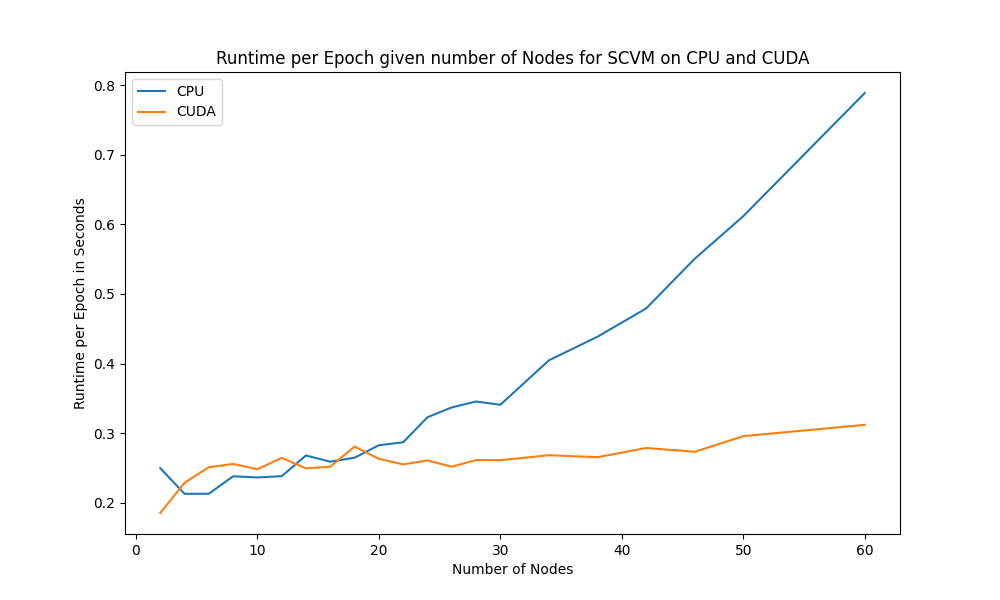
\includegraphics[width=\textwidth]{0_images/numnodes_runtime2.png}
    \caption{Run time of the SCVM relative to the number of nodes $N$}
    \label{fig:NumNodesRuntimes}
\end{figure}
\textbf{Number of Steps}
\\
The second test is carried out in order to evaluate the impact on run time in relation to the number of steps the SCVM has to fit.
For this test, the number of steps is taken from the range:
\begin{equation}
    Num\_Steps = [4,8,12,16,20,30,40,50,75,100,150,200,250,300,350,400,450,500,750,1000]
\end{equation}
The dataset is generated using $\beta = 5.0$ and $N = 4$ nodes, and the resulting dataset has size $n = 5997$.
Again, for each number of steps, the mean run time per epoch over five runs are recorded for both the CPU and CUDA.

Figure \ref{fig:NumStepsRuntimes} below shows the run times per epoch given the number of steps the SCVM has to fit, using the CPU (in blue) and CUDA (in orange).

\begin{figure}[H]
    \centering
    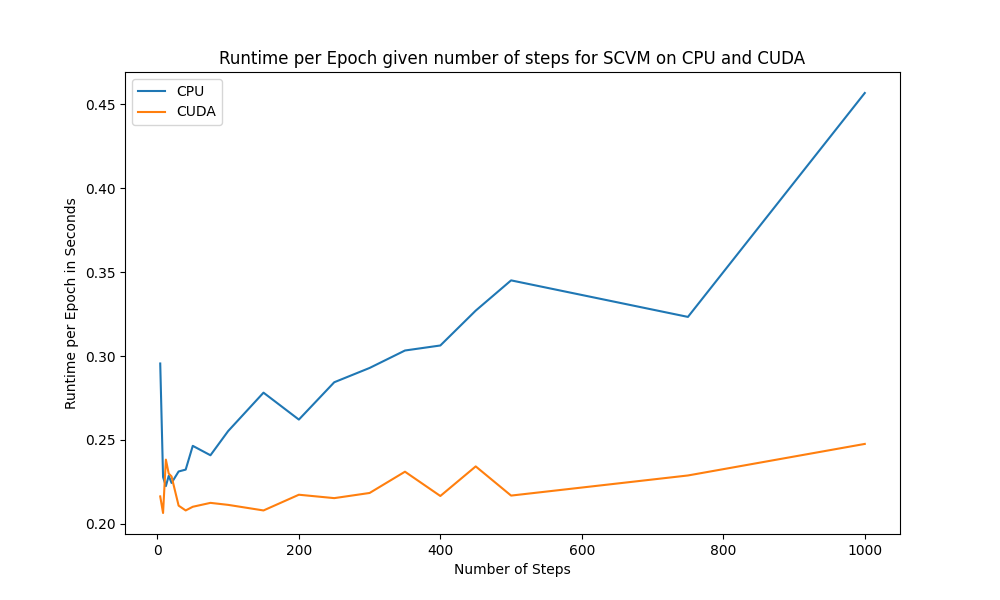
\includegraphics[width=\textwidth]{0_images/steps_runtime2.png}
    \caption{Run time of the SCVM relative to the number of steps}
    \label{fig:NumStepsRuntimes}
\end{figure}
\textbf{Number of Interactions}
\\
The third and final scalability test is carried out with the goal of evaluating the impact on run time the dataset size has.
For this test, the data is generated based on the $\beta$-value, taken from the range:
\begin{equation}
    \beta = [5.0, 5.25, 5.5, 5.75, 6.0, 6.25, 6.5, 6.75, 7.0, 7.25, 7.5, 7.75, 8.0, 8.25, 8.5, 8.75, 9.0]
\end{equation}
The number of interactions generated from these beta values are as follows:
\begin{equation}
    n = 
\end{equation}

The dataset is generated using $N = 4$ nodes, and SCVM has to fit four velocity vectors to each node, ie. four steps.
Once again, for each dataset size, the mean run time per epoch over five runs are recorded for both the CPU and CUDA.

Figure \ref{fig:NumInteractionsRuntimes} below shows the run times per epoch given the number of steps the SCVM has to fit, using the CPU (in blue) and CUDA (in orange).


\begin{figure}[H]
    \centering
    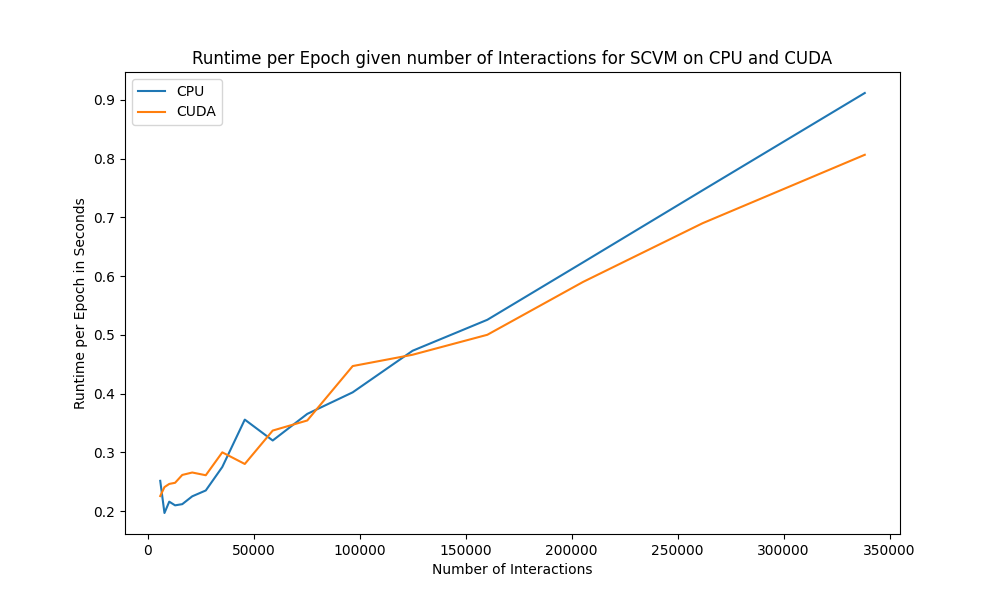
\includegraphics[width=\textwidth]{0_images/numinteractions_runtime2.png}
    \caption{Run time of the SCVM relative to the number of interactions}
    \label{fig:NumInteractionsRuntimes}
\end{figure}
\clearpage
\subsection{Third Research Question}
\label{sec:ResearchQuestion3}
The third research question of this project states:
\\
"How can the model be visualized to enforce explainability?"



\subsubsection{Lyon Primary School dataset}
\label{sec:ResearchQuestion3:LyonDataset}

Real dataset 3, see section \ref{sec:Data:RealData:RealDataset3}, is utilized here.
\\\\
\textbf{Animation check without position correction and discussion.}


\textbf{Animation check with position correction and discussion.}


\textbf{Animation check with regularization and discussion.}




\clearpage

\section{Discussion}


\subsection{Discussion of Results}
\label{sec:DiscussionResults}

%%%%%%%%%%%%%%%%%%%%%%%%%%%%%%%%%%%%%%%%%%%%%%%%%%%%%%%%%%%%%%%%%%%%%%%%%%%%%%%%%%%%%%%%%%
\subsubsection{First Research Question}
\label{sec:DiscussionResults_Q1}



%%%%%%%%%%%%%%%%%%%%%%%%%%%%%%%%%%%%%%%%%%%%%%%%%%%%%%%%%%%%%%%%%%%%%%%%%%%%%%%%%%%%%%%%%%
\subsubsection{Second Research Question}
\label{sec:DiscussionResults_Q2}



%%%%%%%%%%%%%%%%%%%%%%%%%%%%%%%%%%%%%%%%%%%%%%%%%%%%%%%%%%%%%%%%%%%%%%%%%%%%%%%%%%%%%%%%%%
\subsubsection{Third Research Question}
\label{sec:DiscussionResults_Q3}

\clearpage






\section{Conclusion}

During the investigations conducted in this project, the posed research questions were answered and a number of insights were found:
\\\\
First of all, the results regarding research question 1 showed that the proposed SCVM had good modelling performance when comparing modelled intensity rates to ground truth models, and naturally outshone previous work when modelling multi-step, synthetically generated dynamic network data.
The tests of dyad removal and interaction removal revealed less striking performance, which might be resulting from the nature of the synthesized datasets. 
To clearly determine the reason for the low performance, more tests have to be conducted.
Nonetheless, the project concludes that the proposed SCVM, specifically through the introduction of stepwise computation, is able to model the interactions of dynamic networks well, with more detail than previous work.
\\\\
The project sought to implement the proposed model in a scalable manner, and the results presented for research question 2 proved that this was achieved with success.
The training times for the vectorized setup was found to be 32 times faster when fitting four nodes with one step, using the CPU, compared to the baseline non-vectorized setup.
In relation to number of nodes, steps and dataset size, the training run times for the proposed training setup were evaluated when running on either the CPU or the GPU using CUDA.
While the run times grew similarly for larger dataset sizes, increasing either number of nodes or steps showed the significant improvements parallelization provides, as it enables full use of the CUDA system. 
In this regard, the proposed model is definitely scalable in terms of computation.
The project discussed limitations to scalability which arise with memory allocation requirements, but found that several solutions to this limitations could be implemented without changing the SCVM training setup in any significant way.
As such, the project concludes that the SCVM was in fact implemented in a scalable manner, to great extend making the modelling of larger networks feasible.
\\\\
With the proposed SCVM, a goal was to create visualizations that are explainable and interpretable for an observer, as to understand the dynamics of a given network.
The results showed that visualizations of datasets based on real dynamic networks could be made so that the network could be inspected at any given time during its duration.
The results regarding explainability evaluated the impact of applying position, drift and rotation correction as well as regularizing the model.
It was found that position and drift correction immediately made for a more interpretable visualization, while correcting rotation was deemed to be an enhancement which mostly improves comparability between different networks.
While regularization was found to slow the movements of nodes down, it was not found to inherently improve the overall explainability of the modelled dynamic networks used in this project.
The project concludes, that while the visualizations produced by the SCVM could advantageously be expanded as to deliver more information in order to improve explainability, animating entities in a dynamic network as nodes with stepwise constant velocity dynamics allowed for an intuitive interpretation of how the nodes relate over time. 
\\\\
Some possibilities of future expansions to the proposed SCVM were discussed, including the introduction of node-specific and step-specific bias terms, as to possibly model a dynamic network with greater detail.
\\\\
Lastly, the project briefly discussed some possible real life use cases the proposed model could be utilized in, one of these being work flow modelling and optimization at hospitals. 
The project further argued that the SCVM-produced embedding of a given dynamic network could potentially be utilized for some machine learning task. 


\clearpage

%\bibliographystyle{unsrt}
%\bibliography{references}
\printbibliography
\clearpage

\section*{Appendix}
\appendix
%Use appendix by inputting seperate files.
%DO NOT WRITE APPENDIX TEXT DIRECTLY HERE IT WILL BE TOO LONG

%test file to show how to add files to the appendix
%\input{appendix/sanity_check_speakers}



\end{document}
